%\newcommand{\CLASSINPUTbottomtextmargin}{20mm}
\documentclass[conference,a4paper]{IEEEtran}

%\usepackage{showframe}
\usepackage{graphicx}
\usepackage{cleveref}
\usepackage{footnote}
\usepackage{url}
\usepackage[inline]{enumitem}

\newcommand{\citeneeded}{\textsuperscript{{[}citation needed{]}}}
\newcommand{\TC}{tangled commit}
\newcommand{\GCR}{Gerrit Code Review}
\newcommand{\Ep}{Epicea}
\newcommand{\Gr}{Griotte}
\newcommand{\code}[1]{\texttt{#1}}

\title{\Gr{}: Improving Code Review\\with Fine-Grained IDE Events}

\author{\IEEEauthorblockN{Skip~Lentz}\IEEEauthorblockA{EEMCS\\Delft
    University of Technology} \and
  \IEEEauthorblockN{Mart\'{i}n~Dias}\IEEEauthorblockA{RMoD\\INRIA
    Lille-Nord Europe}}

\begin{document}
\maketitle{}
\begin{abstract}
  Code review is a difficult process for multiple reasons:
  \begin{enumerate*}
  \item developers often create \textit{tangled commits},
  \item commits may touch many different parts of a project,
  \item commit messages can be inaccurate or wrong\citeneeded{} and
  \item requesting a review for a change requires too much effort from
    the perspective of the developer.
  \end{enumerate*}

  This work aims to propose a solution to these problems by exploiting
  the information provided by fine-grained IDE events.

  To put this solution in practice, we will develop a code review tool
  named \textit{\Gr} in the \textit{Pharo} environment.
\end{abstract}
\begin{IEEEkeywords}
  code review, fine-grained IDE events, \Ep, \Gr, Pharo
\end{IEEEkeywords}

\section{Problem Description}
\label{sec:problem-description}
Code review is a difficult task for a reviewer to perform, resulting
in loss of time \citeneeded{}. This is partly due to the following two
factors: \TC{}s and the line-based nature of common code review
tools. We will explain the two factors, and how they cause the
difficulty of code review.

\subsection{Tangled Commits}
\label{sec:tangled-commits}
A \TC{} is a commit which is the result of multiple, mutually
unrelated changes. A commit could consist of a refactoring, some
formatting changes, and a change to the body of a method (the latter
being the change for which the commit is actually meant).

This makes it harder to review for obvious reasons. Suddenly, multiple
changes are being treated as one change.

\subsection{Line-based changes}
\label{sec:line-based-changes}
Code review tools often feature a change browser (or \textit{diff
  browser}) with the ability of commenting on lines. One line can
correspond to multiple changes, or vice versa. This is what is meant
by the line-based nature of code review tools.

This is a problem in the case of a tangled commit in which changes
overlap on a single line. If one would comment on that line, it is not
clear to which change it belongs.

\section{Proposed Solution}
\label{sec:proposed-solution}
We propose a solution to this problem by introducing the concept of
groups. A group consists of one or more code changes which are
mutually related, accompanied with a descriptive label. An example
would be the refactoring of a method's name from \code{foo} to
\code{bar}. By grouping changes, we change the perspective from a
\textit{line}-based review tool, to a \textit{change}-based review
tool.

In practice, these groups can be created automatically (as is the case
for refactoring changes), or manually using specially designed tools.

To be able to group code changes, we need fine-grained
information. This information is recorded by --- and collected from
--- \textit{\Ep}, which will be discussed in the next section.

\section{First-Class Code Changes from \Ep}
\label{sec:first-class-ide}
\Ep\ is a Pharo project providing a model for first-class code changes
and related IDE tools. \Ep\ records code changes during development,
allowing us to analyze a more fine-grained history of the
codebase. This is in contrast with the code change information
available from a Version Control System\ (VCS) repository, which is
much more coarse-grained. The model of \Ep\ can be divided into two
parts: \textit{high-level} and \textit{low-level} code changes.

Low-level code changes are additions, deletions or modifications of
program components such as classes or methods. Examples of these code
changes are a method modification, a class addition, etc.

Secondly, \Ep\ records IDE events such as a test run (and its
outcome), refactorings, and loading a version from the VCS. These are
known as high-level code changes.

\Ep\ records this data by means of the \textit{\Ep\ Monitor}, which
listens to events in Pharo as they happen, and converts them to the
first-class code change model objects described above. These objects
are then stored and persisted in a log.

\section{Forming Groups using First-Class Code Changes}
\label{sec:code-review-using}
There are different strategies we can employ to form groups of code
changes. In the simplest sense, they can be formed automatically or
manually. In this section we discuss which strategy --- automatic or
manual --- is the right one for various kinds of groups.

\subsection{Automatically forming groups}
\label{sec:autom-form-groups}
The automatic approach is likely the most suitable for code changes
done by a refactoring. Since refactorings are provided with rich
information in the Epicea model, forming this code change as a group
and creating a descriptive label should be straightforward.

Another approach is comparing the \textit{abstract syntax tree}\ (AST)
to detect whether or not the code change entails a change of behavior
in the program. While the detection of this is straightforward,
creating a descriptive label is less so. For example, both the
addition of a comment and a formatting in the body of a method cause
no change in the AST. Thus, in this case, the labels of the groups
become less descriptive. However, even a non-descriptive label such as
``No change in behavior'' assists the reviewer in understanding the
code more than there being no label at all.

We foresee a challenge in this approach; namely that many changes are
shadowed or undone and thus do not reach the
VCS\cite{Nega12a}. Detecting this is not trivial, but necessary to
reduce the unneeded groups in the output.

\subsection{Manually forming groups}
\label{sec:manu-form-groups}
When groups are formed manually, we have the benefit of being able to
create a very precise label for the group. An obvious downside is that
this requires us to count on the assistance of the developer. A
separate tool for this could therefore prove useful.

An example of such a tool is the \textit{\Ep\ Task
  Clusterer}\cite{Dias15a}, which provides the developer with an
intuitive user interface to group ``tasks''. In this context, a task
refers to the resulting code of resolving an issue or bug-report.

\section{Implementation}
\label{sec:implementation}
We aim to implement a code review tool named \textit{\Gr} for Pharo
which employs the concept of groups. This section aims to present the
implementation of the tool. An important part of the tool is that it
leverages existing services providing code review features such as
\textit{GitHub} or \textit{Gerrit}. See \cref{fig:diagram} for a
simplified diagram of the architecture.
\begin{figure}[t]
  \centering{\resizebox{\linewidth}{!}{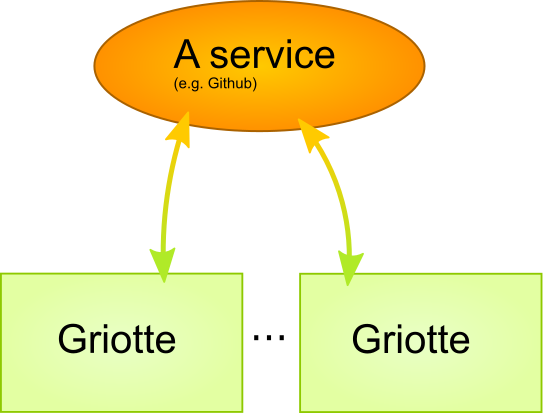
\includegraphics{idea.png}}}
  \caption{Simplified architecture diagram}
  \label{fig:diagram}
\end{figure}

\subsection{Leveraging existing services}
\label{sec:lever-exist-serv}
A key part of our implementation will be the use of existing
services. We discuss the advantages and disadvantages, and how this
approach is to be implemented.

An advantage is that this allows us to alleviate ourselves from part
of the maintenance of the code review tool. This includes both server
maintenance and server-side code maintenance. Furthermore, we get
security and additional functionality for free.

A disadvantage is that we need to sacrifice some of our own
flexibility, and rely on the flexibility of the API's of external
services like GitHub. In a research project this might seem less
ideal, as one would like to be free to explore different
options. However, we feel that we have found the middle way between a
pragmatic solution and a more research oriented solution.

The idea is that the special features which use the concept of groups
are to be accessible only client-side, i.e. from within Pharo. The
information necessary for the groups can be stored as metadata on the
external service. For example, in the case of git-based services such
as GitHub or Gerrit, we can use the
\code{git-notes}\footnote{Documentation:
  \url{http://git-scm.com/docs/git-notes}} model to store metadata on
commits.

\section{Conclusion}
\label{sec:conclusion}
To conclude and summarize, we presented the problems with Modern Code
Review, namely that it does not handle tangled commits, and uses a
line-based approach for review.

We proposed an approach aiming to solve these problems, namely a
change-based form of code review using the concept of groups. The
groups are formed using fine-grained code changes provided by \Ep. We
divided the forming of groups into two categories, automatic and manual.

Furthermore, we presented our proposal for an implementation of a code
review tool using the concept of groups, named \Gr. A key idea of our
implementation is the use of existing external services such as GitHub
and Gerrit. We discussed the benefits and limitations of this
approach.

\bibliographystyle{IEEEtran}
\bibliography{IEEEabrv,rmod,others}
\end{document}

%%% Local Variables:
%%% mode: latex
%%% TeX-master: t
%%% End:
